\begin{ledgroupsized}[r]{120mm}
\footnotesize
\pstart
\noindent\textbf{\"{U}berlieferung:}   
\pend
\end{ledgroupsized}
\begin{ledgroupsized}[r]{114mm}
\footnotesize
\pstart
\parindent -6mm
\makebox[6mm][l]{\textit{L}}Konzept: LH XXXVII 5 Bl. 4-5, 8-9.
2 Bog. 4\textsuperscript{o}.
7 S. und 5 Z.
Am oberen linken Rand von Bl. 4~r\textsuperscript{o} der Vermerk: \textit{De motu cogitata confusanea (1)}.
Am oberen rechten Rand von Bl. 8~r\textsuperscript{o} der Vermerk: \textit{De motu cogitata confusanea (2)}.
Die Zeichnungen [\textit{Fig.~13}] und [\textit{Fig.~14}] sind durch Papierverlust leicht besch\"{a}digt.
Die Bogen, beide durch Papier\-er\-haltungsma{\ss}nahmen gesichert, tragen mittig je ein verschiedenes Wasserzeichen.%
\newline%
Cc 2, Nr. 945 A%
\pend
\end{ledgroupsized}

%\normalsize
\vspace*{5mm}
\begin{ledgroup}
\footnotesize 
\pstart
\noindent\footnotesize{\textbf{Datierungsgr\"{u}nde}: Das vorliegende Stück N.~30 befasst sich versuchsweise mit dem Phänomen der Reibung
als Ursache der Verzögerung sich in widerstehenden Medien bewegender Körper.
Die Thematik wird vorwiegend im Zusammenhang mit theoretischen Ansätzen zum Stoß elastischer Körper
und zu ver\-wandten Phänomenen behandelt.
Hierbei weist N.~30 Berührungspunkte mit den Auszügen aus Wallis' \textit{Mechanica} (N.~8 und N.~9)
sowie insbesondere mit den Auszügen aus Mariottes \textit{De la percussion} (N.~50) auf,
welche insgesamt auf die letzten Monate 1674 und die ersten Monate 1675 datierbar sind.
Ferner unterscheidet sich N.~30 von den eigenhändig auf April 1675 datierten Stücken N.~31 und N.~32 vornehmlich dadurch,
dass in N.~30 noch keine auf die logarithmische Funktion rekurrierende geometrische Beschreibung der % durch die Reibung verursachten 
Verzögerung unternommen wird;
diese Beschreibungsmethode wird indessen in allen späteren Stücken über die Reibung angewendet.
Es liegt demnach nahe, N.~30 für früher als N.~31 und N.~32 zu halten.
Auf Bl.~4-5 kommt zudem das gleiche Wasserzeichen vor wie in N.~31 % (LH XXXVII 5, Bl.~12) 
und in N.~32 (LH XXXVII 5, Bl.~6).
Es ist daher zu vermuten, dass der entsprechende Text nicht viel früher entstanden ist.
Das Wasserzeichen auf Bl.~8-9 dürfte dagegen mit dem unvollständigen Wasserzeichen im späteren Stück N.~38 % (LH XXXVII 5 Bl.~142)
identisch sein. Dies kann als Indiz dafür betrachtet werden,
dass Bl.~4-5 einerseits und Bl.~8-9 andererseits nicht genau zur gleichen Zeit verfasst wurden.
Dementsprechend wird N.~30 in zwei Teile unterteilt.
Ihr enger Zusammenhang zeigt sich aber auch darin,
dass Leibniz die Textträger durchnummeriert und beide mit dem Vermerk \textit{De motu cogitata confusanea} versieht.
Aus den erwähnten Gründen lässt sich annehmen,
dass das Stück N.~30 insgesamt zwischen Anfang und Frühjahr 1675 entstanden ist.}
\pend
\end{ledgroup}

\vspace*{8mm}
\newpage
\pstart
\noindent[4~r\textsuperscript{o}] 
\pend
\pstart
\begin{center}
De Detrimento Motus\protect\index{Sachverzeichnis}{detrimentum motus}, (:~ab attritu\protect\index{Sachverzeichnis}{attritus}, scilicet~:)
 \end{center}
 \pend
 \pstart
\vspace{0,5em}
\begin{center}
 [\textit{Teil 1}] 
\end{center}
\pend
 

\count\Bfootins=1000
\pstart
\noindent
Esto corpus \textit{A} insistens plano in \edtext{\textit{BC}, cui pondere suo innititur. Ponatur impelli recta \textit{DE}}{\lemma{\textit{BC},}\Bfootnote{\textit{(1)}\ impulsum\protect\index{Sachverzeichnis}{impulsus} \textit{(2)}\ linea \textit{(3)}\ cui recta \textit{DE} \textit{(4)}\ cui [...] innititur. \textit{(a)}\ Hoc si \textit{(b)}\ Ponatur [...] \textit{DE}, \textit{L}}}, sentietur aliqua in propellendo \edtext{difficultas. Primum quaestio est, an si}{\lemma{difficultas.}\Bfootnote{\textit{(1)}\ Equidem \textit{(2)}\ Si \textit{(3)}\ Et etsi \textit{(4)}\ Si \textit{(5)}\ Primum [...] si \textit{L}}} planum ponatur esse perfectum atque ita durum, ut planitiei summa aequalitas nullo incumbentis nisu mutari \edtext{possit, difficultas tamen superfutura sit}{\lemma{possit,}\Bfootnote{\textit{(1)}\ difficultatem tamen superare credo \textit{(2)}\ difficultas [...] sit \textit{L}}}, ab ipso illo nisu unionis, quo corpora jungantur. Sed non arbitror, alioqui \edtext{enim in summe politis}{\lemma{enim}\Bfootnote{\textit{(1)}\ summe polita \textit{(2)}\ in summe politis \textit{L}}}, ut glacies maxima onera non 
     \begin{wrapfigure}{l}{0.47\textwidth}                    
     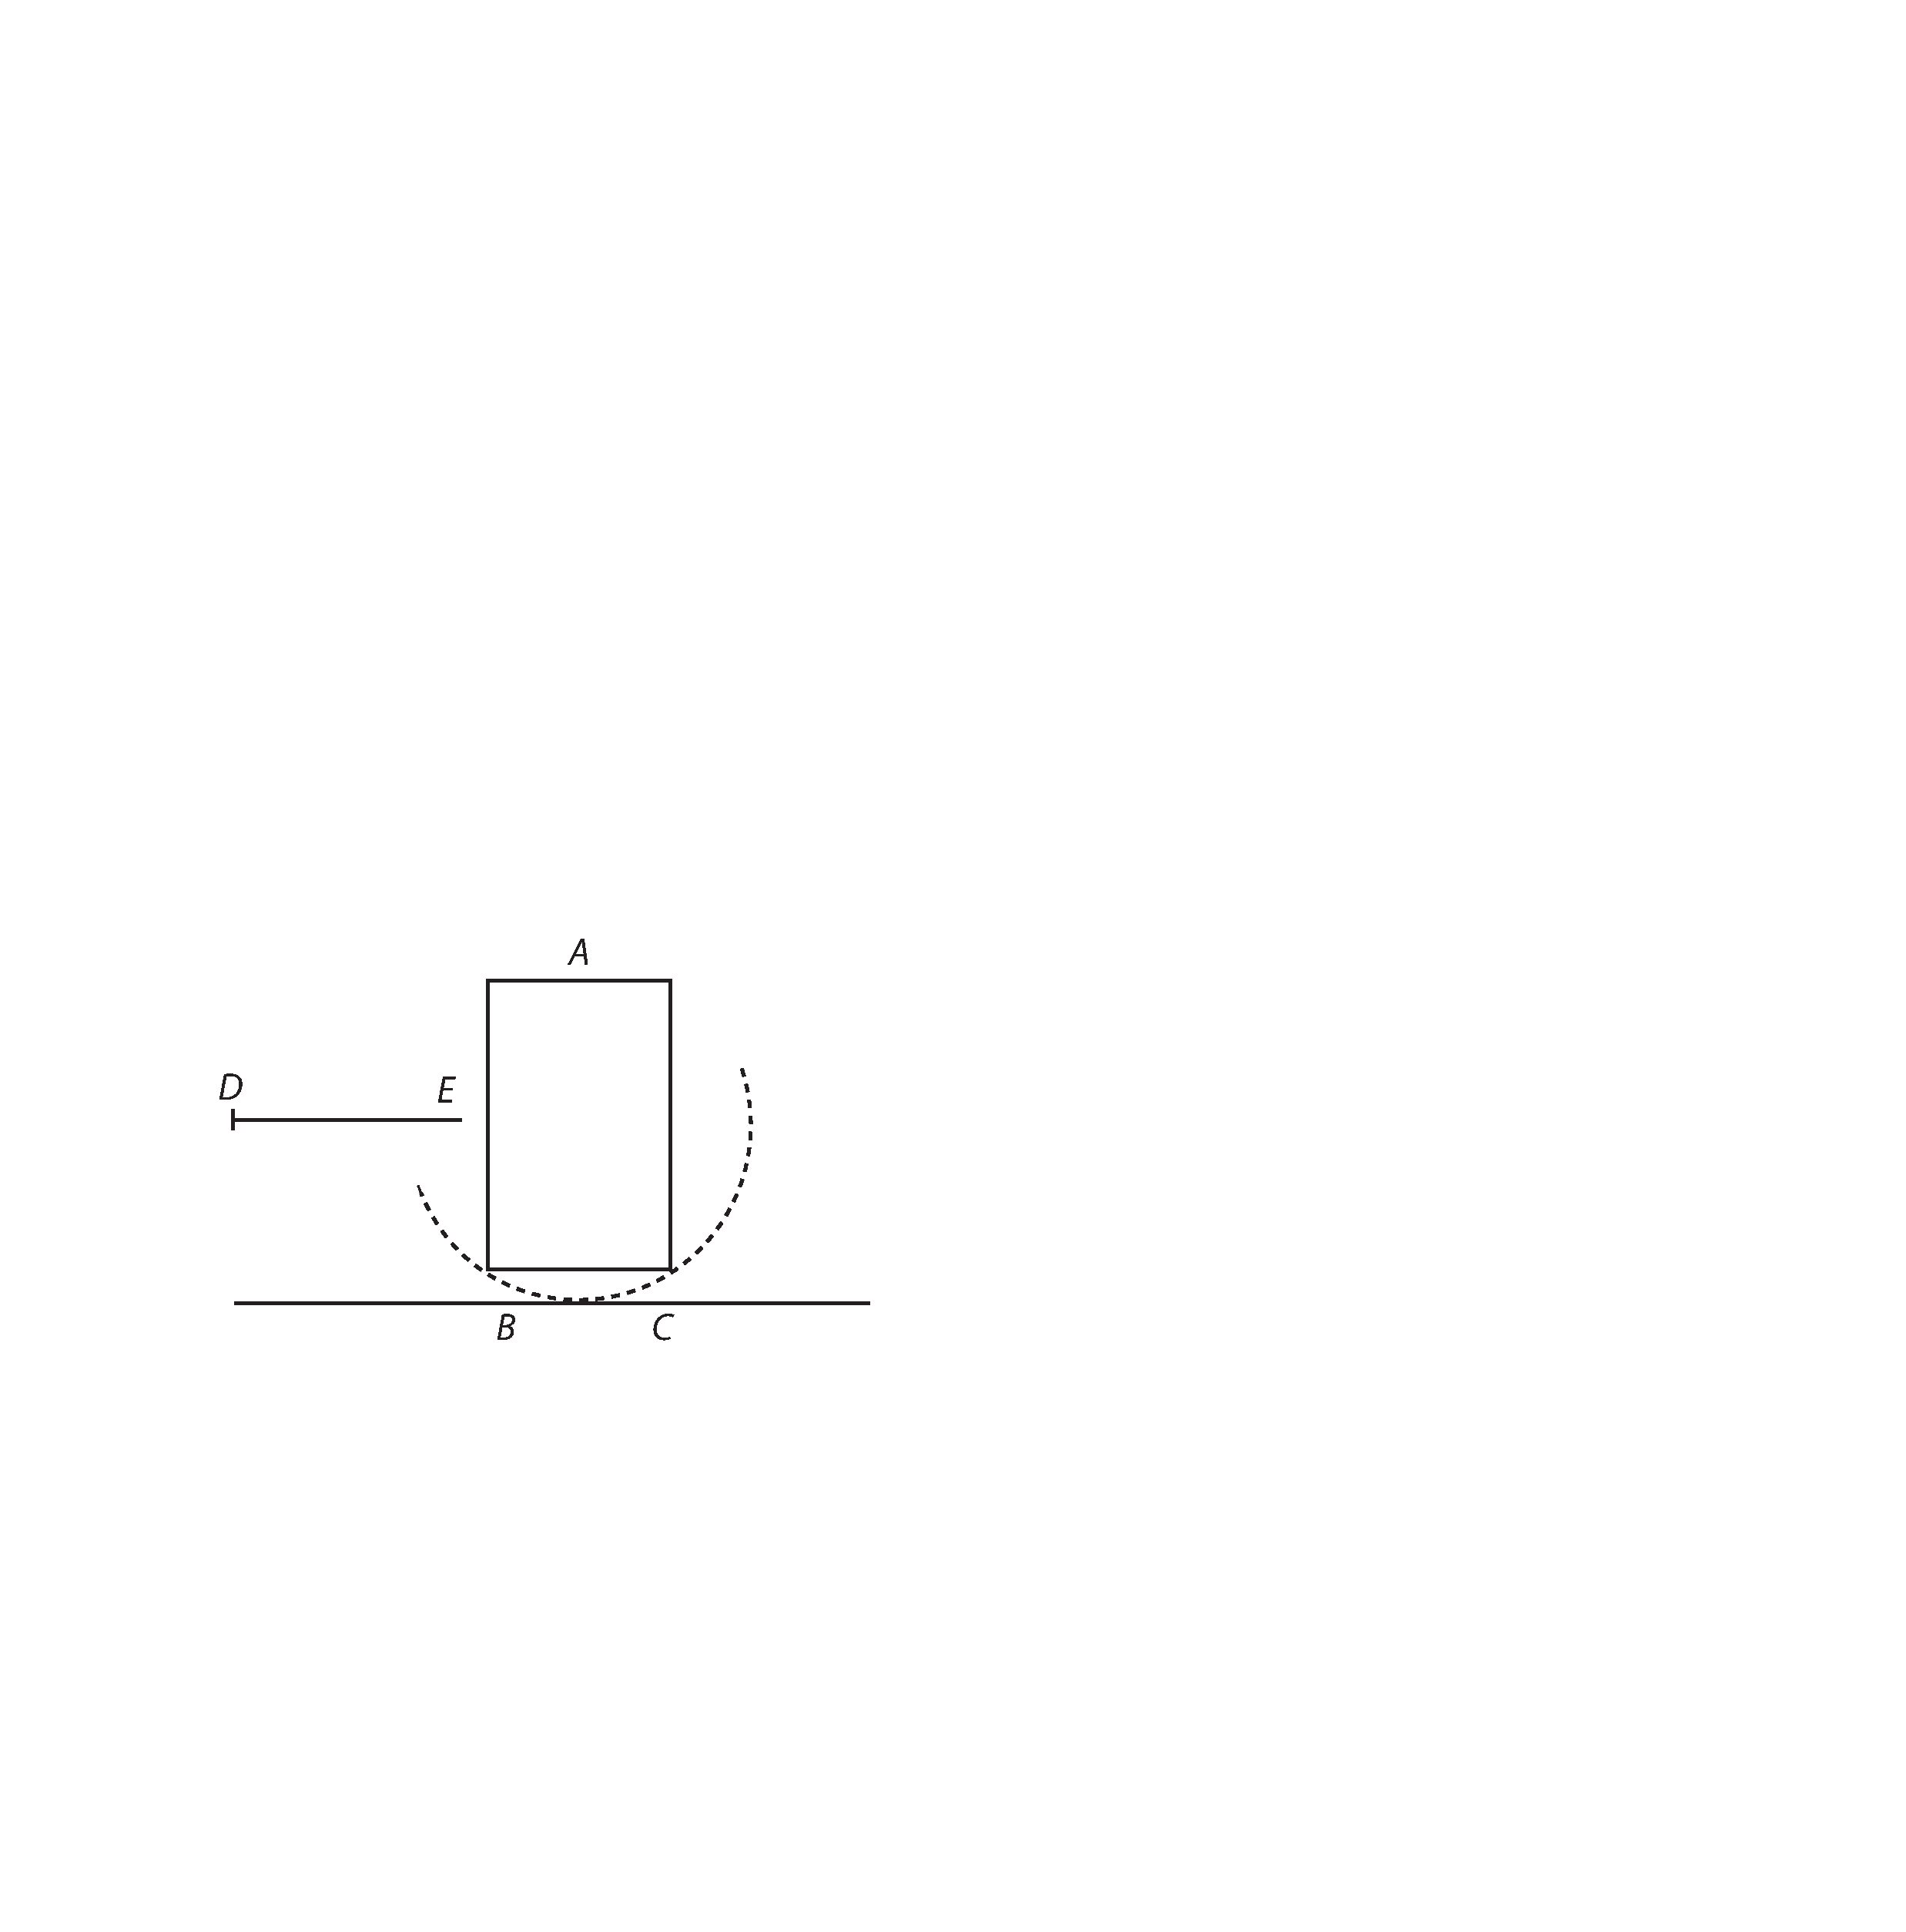
\includegraphics[trim = 48mm 123mm 220mm 205mm, clip, width=0.47\textwidth]{images/lh03705_004r-d1.pdf}
\noindent \centering [\textit{Fig. 1}]
     % \caption{Bildbeschreibung}
     \end{wrapfigure}
\noindent tanta facilitate propellerentur. Et si unionis vis\protect\index{Sachverzeichnis}{vis} a nisu est, tanta foret unio, quantus est nisus, et separare volentibus superandum esset totum corporis pondus\protect\index{Sachverzeichnis}{pondus}, nec facilius esset impellere corpus in glacie aut aqua quam tollere in sublime. Credendum est ergo attritum\protect\index{Sachverzeichnis}{attritus} omnem esse a corporum \edtext{inaequalitate. Aestimanda autem sunt, quantitas contactus, scabrities}{\lemma{inaequalitate.}\Bfootnote{\textit{(1)}\ Pari inaequalitate, sca \textit{(2)}\ Seu scabrities si par est \textit{(3)}\ Seu scabrities \textit{(4)}\ Aestimanda [...] scabrities \textit{L}}}, pondus\protect\index{Sachverzeichnis}{pondus} innitentis, quantitas contactus, nam plurimum interest globum, an cubum propellas; scabrities, nam refert in marmore polito, an in \edtext{tapete globus decurrat;}{\lemma{tapete}\Bfootnote{\textit{(1)}\ globulus \textit{(2)}\ globus \textit{(a)}\ sit \textit{(b)}\ decurrat \textit{L}}} ac pondus\protect\index{Sachverzeichnis}{pondus} innitentis, nam globus ponderosior caeteris paribus non aeque procurret. Sed re recte \edtext{expensa judico, si corpus, ut globulus decurrat super tapete, nihil conferre ejus pondus}{\lemma{expensa}\Bfootnote{\textit{(1)}\ nihil conferre arbitror pondus\protect\index{Sachverzeichnis}{pondus}, nisi ita \textit{(2)}\ judico [...] ejus pondus \textit{L}}} ad \edtext{attritum\protect\index{Sachverzeichnis}{attritus}, sed}{\lemma{attritum,}\Bfootnote{\textit{(1)}\ consideranda semel \textit{(2)}\ sed \textit{L}}} pondus\protect\index{Sachverzeichnis}{pondus} idem agit etiamsi in vacuo moveretur; totam enim vim\protect\index{Sachverzeichnis}{vis} motus statim reducit ad certum moderamen: eaque vis\protect\index{Sachverzeichnis}{vis} obstaculo aliquo recepto, et saepe continuato ut quando in tapete decurrit continue decrescit. Perinde ac \edtext{si}{\lemma{}\Bfootnote{si  \textbar\ in \textit{streicht Hrsg.}\ \textbar\ corpus \textit{L}}} corpus in media aqua \edtext{procurrat. Idem}{\lemma{procurrat.}\Bfootnote{\textit{(1)}\ Sed ita \textit{(2)}\ Idem \textit{L}}} est \edtext{quando globum ponimus}{\lemma{quando}\Bfootnote{\textit{(1)}\ corpus poni \textit{(2)}\ globum ponimus \textit{L}}} decurrere in tabula glutinosa. Sed quando ponimus tabulam esse inaequalem, pondus\protect\index{Sachverzeichnis}{pondus} corporis ad rem pertinere arbitror; majore enim vi\protect\index{Sachverzeichnis}{vis} opus est, ad elevandum corpus, ut exiguum quendam montem superet, quam ad ipsum a glutine avellendum. Ibi enim glutinis tantum vis\protect\index{Sachverzeichnis}{vis} superatur, et corporis in quantum motui in plano resistit pondus\protect\index{Sachverzeichnis}{pondus} ejus. Hic vero ipsum corporis pondus\protect\index{Sachverzeichnis}{pondus}, idem est de alio nisu corporis contra aliud corpus quod contingit, ut chordarum contra rotas. Excutiendum tamen obiter est, antequam \edtext{pergamus, unde}{\lemma{pergamus,}\Bfootnote{\textit{(1)}\ an \textit{(2)}\ unde \textit{L}}} fiat, ut corpus in plano etiam politissimo videatur difficulter propelli posse. Ego non video unde ea resistentia\protect\index{Sachverzeichnis}{resistentia} oriri possit, nisi ab eo qui superest attritu\protect\index{Sachverzeichnis}{attritus}, contra aerem \edtext{planum}{\lemma{}\Bfootnote{planum \textit{erg.} \textit{L}}} et alia corpora per quae decurrit. Pone sagittam\protect\index{Sachverzeichnis}{sagitta} horizontaliter projici, pondus\protect\index{Sachverzeichnis}{pondus} eam tandem ad terram deducit, ita pondus\protect\index{Sachverzeichnis}{pondus} vehae, sive d'un traîneau agens contra inaequalitates glaciei tandem vim\protect\index{Sachverzeichnis}{vis} impressam destruit. Quod longius projicimus pilam\protect\index{Sachverzeichnis}{pila} plumbeam \edtext{quam ligneam,}{\lemma{quam}\Bfootnote{\textit{(1)}\ aeneam, \textit{(2)}\ ligneam, \textit{L}}} ratio esse videtur, quod plumbum\protect\index{Sachverzeichnis}{plumbum} solidius, unde minus in eo materiae extraneae, sive aethereae atque ideo minus attritus\protect\index{Sachverzeichnis}{attritus}, quemadmodum chartam in globulum\protect\index{Sachverzeichnis}{globulus} compressam longius projeceris, quam \edtext{expansam, aut}{\lemma{expansam,}\Bfootnote{\textit{(1)}\ quia \textit{(2)}\ at \textit{(3)}\ aut \textit{L}}} 
\count\Bfootins=1500
ne huic exemplo \edtext{chartae}{\lemma{}\Bfootnote{chartae \textit{erg.} \textit{L}}} latitudinem objicias, longius projicies spongiam compressam, quam dilatatam. Et sane ab ejusmodi detrimento\protect\index{Sachverzeichnis}{detrimentum} oriri pendulorum\protect\index{Sachverzeichnis}{pendulum} et Elateriorum cessationem, aut certe detrimentum\protect\index{Sachverzeichnis}{detrimentum}, videtur manifestum. Satis ergo fortis causa ad rationem reddendam, cur corpora majora difficilius impellantur. Videmus ergo ab Attritu\protect\index{Sachverzeichnis}{attritus} oriri magnorum phaenomenorum% \pend